%======================================================================
\section{Guía de esta parte: cinco maneras de tratar el riesgo}\label{sec:riesgo-guia}
%======================================================================
Las partes~IV y~V trataron el MPC como un problema \emph{determinista}: dada la fuga
pronosticada, elegir el caudal del ACS que mantiene la PCT en la consigna. Esta parte agrega lo
que el MPC determinista no ve: que el ACS puede fallar, que no se sabe cuándo ni por cuánto
tiempo, y que una falla larga puede llevar la PCT sobre 1220~K. El plan del proyecto
(\code{docs/monolithic\_formulation\_plan.md}, §7 y §8.11--8.18) ordenó las maneras de
incorporar ese riesgo de menor a mayor complejidad. La figura~\ref{fig:riesgo-escalera} las
muestra como una escalera, y la tabla~\ref{tab:riesgo-guia} dice dónde está cada una en el
plan y en este documento.

\begin{figure}[H]\centering
\resizebox{\linewidth}{!}{%
\begin{tikzpicture}[
  st/.style={draw=accent, line width=0.6pt, rounded corners=2pt, fill=soft, align=center,
             font=\small, minimum height=19mm, text width=29mm, inner sep=2pt},
  fut/.style={st, fill=white, dashed},
  arr/.style={-{Stealth[length=2mm]}, line width=0.7pt, draw=ink},
  lab/.style={font=\scriptsize, text=black!65, align=center}]
\node[st] (n0) at (0,0)    {\textbf{0. Determinista}\\sin métrica\\N1, N2, N3\\límite $U_y$ blando};
\node[st] (n1) at (3.6,0.9)  {\textbf{1. Margen}\\\textbf{determinista}\\DSM de la tesis};
\node[st] (n2) at (7.2,1.8) {\textbf{2. Métrica}\\\textbf{probabilística}\\cuantil, CVaR, Wilks,\\pérdida esperada};
\node[st] (n3) at (10.8,2.7){\textbf{3. Escenario}\\\textbf{único}\\Homem-de-Mello,\\estrategia de Rozas};
\node[fut] (n4) at (14.4,3.6){\textbf{4. Multietapa}\\(futuro)\\árbol de modos del\\ACS, recurso real};
\draw[arr] (n0) -- (n1); \draw[arr] (n1) -- (n2); \draw[arr] (n2) -- (n3); \draw[arr] (n3) -- (n4);
\node[lab, below=1.5mm of n0] {no ve la falla;\\se prueba \emph{a posteriori}};
\node[lab, below=1.5mm of n1] {ve la predicción\\nominal, no la falla};
\node[lab, below=1.5mm of n2] {ve la distribución\\de la duración};
\node[lab, below=1.5mm of n3] {la misma decisión con\\un solo escenario};
\node[lab, below=1.5mm of n4] {decisiones que se\\adaptan al modo del ACS};
\end{tikzpicture}}
\caption{La escalera del riesgo. Cada peldaño agrega información sobre la incertidumbre al
problema de optimización. Los peldaños 0--3 están implementados y medidos en lazo cerrado; el 4
es una línea futura (sección~\ref{sec:riesgo-futuro}).}
\label{fig:riesgo-escalera}
\end{figure}

\begin{table}[H]\centering\footnotesize\setlength{\tabcolsep}{3pt}
\begin{tabularx}{\linewidth}{@{}>{\raggedright\arraybackslash}p{27mm} >{\raggedright\arraybackslash}p{30mm} Y >{\raggedright\arraybackslash}p{24mm}@{}}\toprule
Peldaño & Fase del plan & Qué se hizo & Dónde\\\midrule
0. Determinista & F2--F3, F5a, F6 & N1, N2, N3 en lazo abierto y cerrado; pruebas con fallas del ACS (familia extrema, fallas del DET en el lazo) & secciones~\ref{sec:niveles}, \ref{sec:extremos}, \ref{sec:riesgo-fallas}\\
1. Margen determinista & F5b.1b, F5b.1b0 & Penalización DSM de la tesis, barrido de $\lambda_{\rm dsm}$, umbral y límite & sección~\ref{sec:dsm-lambda}\\
2a. Riesgo de pronóstico & F4 & Restricción probabilística gaussiana y SAA de dos etapas con 59 trayectorias de fuga (N3) & sección~\ref{sec:riesgo}\\
2b. Riesgo de fallas del ACS & F5b.1c, F5b.1d, F6, F8 & Cota con cuantil, CVaR, Wilks 59, pérdida esperada (SAA), fallas parciales; estimador de Rao--Blackwell; supresión $R$ & secciones~\ref{sec:riesgo-cota}--\ref{sec:supresion}\\
3. Escenario único & V6, F9 & Teorema de Homem-de-Mello et al.; escenario aprendido según el contexto & sección~\ref{sec:rozas}\\
4. Multietapa & V8, V9 (ruta) & No implementado; formulación y condiciones en que valdría la pena & sección~\ref{sec:riesgo-futuro}\\\bottomrule
\end{tabularx}
\caption{Dónde está cada peldaño en el plan del proyecto (\code{docs/implementation\_route.md},
vías V6--V9) y en este documento.}
\label{tab:riesgo-guia}
\end{table}

\paragraph{Cómo leer esta parte.} Primero se explican las métricas desde cero, con un ejemplo de
juguete que se resuelve a mano (sección~\ref{sec:riesgo-metricas}), y luego cómo se calcula
cada una en una consulta real del SMDFR (sección~\ref{sec:riesgo-calculo}). La
sección~\ref{sec:riesgo-teoremas} reúne los teoremas en que se apoya cada caso y lo que implican.
La sección~\ref{sec:riesgo-como-entra} escribe cada formulación como una modificación explícita
de N2. Siguen los experimentos, en el orden en que se hicieron
(secciones~\ref{sec:riesgo-donde}--\ref{sec:trayectorias}), y al final una síntesis que ordena
todos los resultados de lo determinista a lo probabilístico
(sección~\ref{sec:riesgo-sintesis}) y los problemas abiertos (sección~\ref{sec:riesgo-futuro}).

%======================================================================
\section{Las métricas de riesgo desde cero}\label{sec:riesgo-metricas}
%======================================================================

\subsection{Qué es el riesgo en este problema}
\paragraph{El evento.} Lo que se quiere evitar es que la PCT cruce $U=1220$~K, el estado final
del árbol de eventos del DET (sección~\ref{sec:extremos}). El límite $U_y=1244$~K de la función
de costo queda más allá y nunca se acerca.

\paragraph{La causa.} El MPC enfría inyectando plomo con el ACS. Si el ACS falla, el caudal es
cero haga lo que haga el controlador, y la PCT sube a razón de unos 0.3~K/s hasta que el ACS se
recupera. Hay tres cantidades aleatorias: \emph{cuándo} empieza la falla, \emph{cuánto} dura
($D$) y, si es parcial, \emph{qué fracción} del caudal se pierde ($\eta$). Otras
incertidumbres, como el error de pronóstico de la fuga o el desajuste entre el ROM y la planta,
resultaron despreciables frente a ésta (secciones~\ref{sec:riesgo} y~\ref{sec:f45}).

\paragraph{La probabilidad que se mide.} Se usan dos versiones:
\begin{itemize}
  \item $P(\text{cruce}\mid\text{falla})$: la probabilidad de cruzar 1220~K \emph{dado} que una
        falla del ACS empieza en un instante del transitorio. Es la que controla la capa de riesgo,
        y no depende de cuán frecuentes sean las fallas.
  \item $P(\text{cruce por transitorio})=P(\text{alguna falla})\times P(\text{cruce}\mid\text{falla})$.
        Es la que interesa al análisis probabilístico de seguridad (APS). Con las tasas aceleradas,
        $P(\text{alguna falla en 220 s})=1-e^{-0.0016\cdot220}\approx0.30$.
\end{itemize}

\paragraph{La palanca.} Durante la falla el controlador no puede hacer nada. Lo único que puede
decidir es en qué estado la recibe: si la PCT está $e$~K bajo la consigna cuando la falla empieza,
la falla tiene que durar $e/0.3$~s más para llevarla a 1220~K. A eso se le llama
\textbf{pre-enfriar}, y su costo es el error de seguimiento y la masa de plomo adicional. Toda
métrica de riesgo de esta parte es, en el fondo, una regla para elegir $e$.

\subsection{El ejemplo de juguete}\label{sec:riesgo-juguete}
Todas las métricas se pueden calcular a mano en un modelo de un paso, el mismo del
ejemplo~\ref{ej:juguete}:
\begin{itemize}
  \item la consigna es $y_{\rm ref}=1179$~K; sin pre-enfriar, el margen hasta 1220~K es
        $m_0=41$~K, y con pre-enfriamiento $e$ es $m=41+e$;
  \item la falla dura $D\sim\mathrm{Exp}$ de media 46~s, y la PCT sube $Z=0.3D$~K; entonces $Z$ es
        exponencial de media $\theta=0.3\cdot46=13.8$~K;
  \item el costo de pre-enfriar es $e^2$ (el error de seguimiento, al cuadrado).
\end{itemize}
La herramienta central es la \textbf{función de supervivencia} del calentamiento,
\[
P(Z>m)=e^{-m/\theta}=e^{-m/13.8}.
\]
Con el margen de la consigna, $P(Z>41)=e^{-2.97}=0.051$: una de cada veinte fallas cruza 1220~K.

\subsection{Las métricas que deciden}\label{sec:riesgo-metricas-decision}
\paragraph{(0) Sin métrica: el MPC determinista.} N1, N2 y N3 predicen la PCT con la fuga
pronosticada y \emph{sin falla}. En el juguete, la predicción es 1179~K, bajo el límite, así que
no hay nada que corregir: $e=0$ y el riesgo queda en 0.051. El MPC determinista no ignora el
riesgo por descuido; simplemente no está en su modelo. Su protección viene de la distancia entre
la consigna y el límite, un \emph{margen implícito} de 41~K que nadie calibró en probabilidad.

\paragraph{(1) Margen determinista (DSM de la tesis).} La tesis agrega
$\lambda_{\rm dsm}\sum_k[\mathrm{DSM}_k-\tau]_+^2$, con
$\mathrm{DSM}_k=(\hat y_k-y_{\rm ref})/(U-y_{\rm ref})$ y $\tau=0.00238$. En el juguete
$\mathrm{DSM}=0$ y el término vale cero: con $U=1244$~K sólo se activa si la PCT \emph{predicha}
supera la consigna en $0.00238\cdot65=0.15$~K. Como la predicción no contiene la falla, el DSM
tampoco la ve. Si se pusiera el umbral bajo la consigna ($\tau<0$), el término empujaría la PCT a
$y_{\rm ref}+\tau(U-y_{\rm ref})$: equivale a correr la consigna una cantidad fija, que no depende de
cuán probable o larga sea la falla.

\paragraph{(2) El PSM de la tesis, como métrica de evaluación.} La tesis calculaba, \emph{después}
de decidir, $\mathrm{PSM}=(U-q_{0.95}[\text{PCT pico}])/(U-y_{\rm nom})$. En el juguete,
$q_{0.95}[\text{pico}]=1179+\theta\ln20=1179+41.3=1220.3$~K. Con $U=1244$~K y $y_{\rm nom}=1179$~K,
$\mathrm{PSM}=23.7/65=0.36$; con $U=1220$~K, $\mathrm{PSM}=-0.3/41<0$: el 5\,\% peor de las fallas
cruza. Observe que $\mathrm{PSM}_{1220}\ge0$ equivale a $q_{0.95}[\text{pico}]\le1220$, es decir, a
$P(\text{cruce}\mid\text{falla})\le0.05$. El PSM es la métrica (3) con $\alpha=0.05$, calculada
tarde.

\paragraph{(3) Probabilidad de cruce: la cota con cuantil.} Se exige
$P(\text{cruce}\mid\text{falla})\le\alpha$. Como $P(Z>m)$ decrece con $m$, la condición equivale a
un margen mínimo:
\[
e^{-m/\theta}\le\alpha\iff m\ge\theta\ln(1/\alpha)=\mathrm{VaR}_{1-\alpha}(Z).
\]
Con $\alpha=0.05$: $m\ge41.3$~K, $e=0.3$~K (casi gratis). Con $\alpha=0.02$: $m\ge54.0$~K, $e=13.0$~K.
La restricción \emph{probabilística} se convirtió en una restricción \emph{determinista} sobre la
PCT antes de la falla: $\mathrm{PCT}\le U-\mathrm{VaR}_{1-\alpha}(Z)$. A esa resta se le llama
\emph{back-off}, y es la idea de la proposición~\ref{prop:margen}(a).

\paragraph{(4) CVaR: controlar la severidad de la cola.} El VaR mira cuántas fallas cruzan; el
CVaR$_\beta$ mira \emph{cuánto} calientan en promedio las peores $(1-\beta)$. Para una exponencial,
$\mathrm{CVaR}_\beta(Z)=\mathrm{VaR}_\beta(Z)+\theta$ (por la falta de memoria: pasado el cuantil, lo
que queda tiene la misma media). Con $\beta=0.95$: $41.3+13.8=55.1$~K, $e=14.1$~K y
$P=e^{-55.1/13.8}=0.018$. El CVaR$_{0.95}$ protege como un cuantil con $\alpha\approx0.018$; en el
SMDFR, como uno con $\alpha\approx0.015$ (sección~\ref{sec:riesgo-formulaciones}).

\begin{ejemplo}[CVaR con diez escenarios y la fórmula de Rockafellar--Uryasev]\label{ej:ru}
Sean diez fallas igualmente probables que calientan
$Z\in\{2,4,6,8,10,12,15,20,30,50\}$~K y $\beta=0.8$. El VaR$_{0.8}$ es el menor valor con
probabilidad acumulada $\ge0.8$: 20~K. El CVaR$_{0.8}$ es el promedio del 20\,\% peor:
$(30+50)/2=40$~K. Rockafellar y Uryasev~\cite{rockafellar2000} mostraron que también es
\[
\mathrm{CVaR}_\beta(Z)=\min_\gamma\Big\{\gamma+\tfrac{1}{1-\beta}\,\mathbb E\big[(Z-\gamma)_+\big]\Big\}.
\]
Con $\gamma=20$: $20+5\cdot(0.1\cdot10+0.1\cdot30)=40$; con $\gamma=15$: $15+5\cdot5.5=42.5$. El mínimo es
40 y se alcanza en el VaR. La ventaja de esta forma es que $(Z-\gamma)_+$ se escribe con una
holgura por escenario, $v_s\ge Z_s-\gamma$, $v_s\ge0$: el CVaR entra en un QP como restricciones
lineales. Si la PCT antes de la falla es $y$, el pico es $y+Z$ y
$\mathrm{CVaR}_\beta(y+Z)=y+40$: el CVaR del pico es la PCT más una constante. Ésa es la
\emph{invariancia a traslaciones}, y es la razón por la que el CVaR también se reduce a un margen.
\end{ejemplo}

\paragraph{(5) El PSM de Wilks en línea.} Se sortean $n=59$ duraciones, se toma la mayor,
$D_{\max}$, y se exige $\mathrm{PCT}\le U-0.3D_{\max}$. Por la regla de Wilks
(proposición~\ref{prop:wilks}), $D_{\max}$ supera el cuantil 0.95 con probabilidad
$1-0.95^{59}=0.952$: la cota garantiza $P\le0.05$ con confianza 95\,\%. Pero el nivel que se
obtiene es aleatorio: $S(D_{\max})$, la probabilidad de que una falla dure más que $D_{\max}$, es el
mínimo de 59 uniformes, con media $1/60=0.017$. En el juguete, el margen cae en el 80\,\% de las
consultas entre 45 y 87~K (mediana 61~K), y cambia de una consulta a la siguiente porque cada una
sortea su muestra. En promedio protege como un cuantil con $\alpha\approx0.017$, pero con ruido
(figura~\ref{fig:riesgo-tutorial}a, banda violeta).

\paragraph{(6) Pérdida esperada.} En lugar de una cota, se penaliza el exceso esperado sobre
1220~K con un peso $\rho$:
\[
J(e)=e^2+\rho\,\mathbb E\big[(Z-m)_+\big]=e^2+\rho\,\theta\,e^{-(41+e)/\theta}.
\]
Al derivar, $2e=\rho\,e^{-(41+e)/\theta}$. Con $\rho=100$, $e^*=2.2$~K y $P=0.044$; con $\rho=1000$,
$e^*=11.3$~K y $P=0.023$. No hay un $\alpha$: el nivel de riesgo sale del equilibrio entre el costo
de pre-enfriar y el precio $\rho$ de cada kelvin de exceso. En el SMDFR se calcula con 40
escenarios de duración (una SAA), porque $\mathbb E[(Z-m)_+]$ no tiene fórmula cerrada para la
mezcla del DET.

\paragraph{(7) El escenario único.} Cada una de las métricas anteriores terminó en un margen
$m$. Entonces existe una duración determinista $D^*$ con $0.3D^*=m$, y el MPC determinista que
«pronostica» una falla de $D^*$ segundos toma la misma decisión. Para el cuantil con
$\alpha=0.02$, $D^*=q_{0.98}(D)=46\ln50=180$~s; para la pérdida esperada con $\rho=100$,
$D^*=(41+2.2)/0.3=144$~s. Ninguna es la duración media (46~s), que no pre-enfría. Es el resultado de
Homem-de-Mello et al.\ en su forma más simple (proposición~\ref{prop:margen}(b) y
sección~\ref{sec:rozas}).

\begin{table}[H]\centering\small
\begin{tabularx}{\linewidth}{@{}Y r r r r@{}}\toprule
Métrica (juguete) & Margen $m$ [K] & Pre-enfriamiento $e$ [K] & $P(\text{cruce}\mid\text{falla})$ & Escenario $D^*$ [s]\\\midrule
(0) Determinista, sin métrica & 41.0 & 0 & 0.051 & ---\\
(1) DSM de la tesis ($\tau=0.00238$) & 41.0 & 0 & 0.051 & ---\\
(3) Cuantil, $\alpha=0.05$ & 41.3 & 0.3 & 0.050 & 138\\
(6) Pérdida esperada, $\rho=100$ & 43.2 & 2.2 & 0.044 & 144\\
(6) Pérdida esperada, $\rho=1000$ & 52.3 & 11.3 & 0.023 & 174\\
(3) Cuantil, $\alpha=0.02$ & 54.0 & 13.0 & 0.020 & 180\\
(4) CVaR$_{0.95}$ & 55.1 & 14.1 & 0.018 & 184\\
(5) Wilks 59 (mediana; 80\,\% central) & 61 (45--87) & 20 (4--46) & 0.012 (0.002--0.038) & 205\\\bottomrule
\end{tabularx}
\caption{Las métricas del juguete, ordenadas por margen. Todas eligen un margen; difieren en la
regla con que lo eligen. La última columna es el escenario único equivalente, $D^*=m/0.3$.}
\label{tab:riesgo-juguete}
\end{table}

\begin{figure}[H]\centering
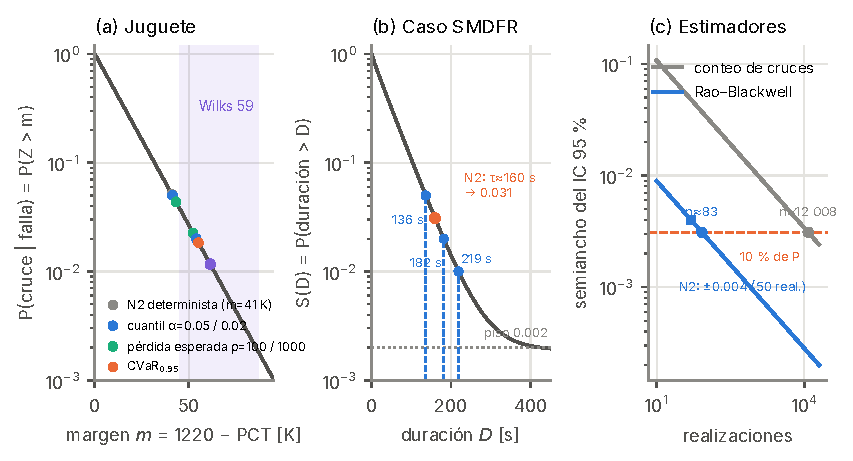
\includegraphics[width=\linewidth]{figures/fig_risk_tutorial.pdf}
\caption{(a) Juguete: probabilidad de cruzar 1220~K en función del margen con que la PCT recibe
la falla. Cada métrica es un punto de la misma curva (el punto gris del MPC determinista queda
bajo el azul del cuantil $\alpha=0.05$); la banda violeta es el 80\,\% central del margen de Wilks
59 y el punto, su mediana. (b) Caso SMDFR: supervivencia de la duración de una falla del ACS
(mezcla del DET acelerada) y los cuantiles que usa la cota; N2 sin capa de riesgo opera con
$\tau\approx160$~s hasta 1220~K y deja $S(160)=0.031$; la componente de 2.9~h fija un piso de 0.002.
(c) Semiancho del intervalo de confianza de $P(\text{cruce}\mid\text{falla})\approx0.031$ según el
número de lazos simulados: contando cruces hacen falta unas 12\,000 realizaciones para un error
relativo del 10\,\%; con Rao--Blackwell, unas 83 (\code{python/make\_risk\_tutorial\_figures.py}).}
\label{fig:riesgo-tutorial}
\end{figure}

\takeaway{\textbf{Lo que muestra el juguete.} Como el pico es «PCT antes de la falla más un
calentamiento que no depende de la decisión», toda métrica de riesgo se convierte en un margen
sobre la PCT. El cuantil lo elige por probabilidad, el CVaR por severidad, Wilks con una muestra
aleatoria y la pérdida esperada por un precio. El MPC determinista y el DSM dejan el margen que
da la consigna, 41~K, sin saber qué probabilidad compra.}

\subsection{Las métricas que evalúan}\label{sec:riesgo-metricas-evaluacion}
Decidir con una métrica no basta: hay que medir, sobre la planta, si la decisión cumplió. Para
eso se usan tres grupos de métricas, siempre con los mismos números aleatorios para todos los
controladores.

\paragraph{Riesgo medido: conteo y Rao--Blackwell.} La forma ingenua es simular $n$ lazos con
fallas y contar cuántos cruzan. Su error estándar es $\sqrt{p(1-p)/n}$: con $p=0.031$ y $n=50$, el
intervalo del 95\,\% es $\pm0.048$, más grande que la probabilidad misma. Con 0 cruces en 60
lazos sólo se puede decir que $p<0.06$. El estimador de Rao--Blackwell
(sección~\ref{sec:riesgo-rb}) no sortea la duración: simula el lazo sin fallas y, en cada instante
$t$, calcula sobre la planta el tiempo $\tau(x_t)$ que tardaría la PCT en llegar a 1220~K si el
ACS fallara ahí. Una falla que empieza en $t$ cruza si y sólo si dura más que $\tau(x_t)$, y esa
probabilidad se conoce exactamente: $S(\tau(x_t))$.

\begin{ejemplo}[Rao--Blackwell con tres lazos]\label{ej:rb}
Suponga tres lazos de N2 con $\tau=130$, 160 y 190~s en el instante de la falla, y duración
$\mathrm{Exp}(46~\text{s})$. Contando, cada lazo aporta un 0 o un 1, y con tres lazos lo más
probable es ver 0 cruces: el estimador vale 0. Con Rao--Blackwell, cada lazo aporta
$S(\tau)=e^{-\tau/46}$: 0.059, 0.031 y 0.016, cuyo promedio, 0.035, ya está cerca del valor
verdadero. La varianza del conteo es $p(1-p)\approx0.034$ por lazo; la de Rao--Blackwell es la
de los tres números, $\approx0.0004$, unas 80 veces menor. Por el teorema de Rao--Blackwell, reemplazar
el indicador del cruce por su esperanza condicional dada la trayectoria no cambia la media y no
aumenta la varianza~\cite{casella2002}. En el SMDFR, la reducción permitió medir
$0.031\pm0.004$ con 50 lazos (figura~\ref{fig:riesgo-tutorial}c).
\end{ejemplo}

\paragraph{Desempeño: las métricas de la tesis.} IAE, tiempo de asentamiento, sobrepaso,
error estacionario, variación total del caudal y DSM mínimo (definidas en la
sección~\ref{sec:desempeno}). Hay que leerlas con cuidado en las capas de riesgo: una capa que
pre-enfría trabaja a propósito bajo la consigna, y el IAE cuenta ese margen como error.

\paragraph{El precio de la prudencia.} El pre-enfriamiento medio (K bajo $y_{\rm ref}$), la masa
de plomo adicional y, en F9, el \emph{valor de la solución estocástica} (VSS): cuánto costo
esperado se ahorra decidiendo con la distribución en vez de con el pronóstico nominal. Una capa de
riesgo se juzga por su posición en el plano riesgo--pre-enfriamiento: dos formulaciones son
equivalentes si caen en el mismo punto de la misma curva.

%======================================================================
\section{Del juguete al SMDFR: cómo se calcula cada métrica en una consulta}\label{sec:riesgo-calculo}
%======================================================================
El juguete tiene una sola falla, exponencial, y un calentamiento lineal. El caso de estudio tiene
cinco componentes, un calentamiento que depende del estado, 26 pasos de horizonte y una planta
distinta del modelo de predicción. Esta sección recorre lo que hace el código en cada consulta
(\code{julia/ClosedLoop.jl}, \code{julia/F6Tasks.jl}).

\paragraph{Paso 0 (una vez): la distribución de la duración.} El ACS tiene cinco componentes en
serie, cada uno una cadena de Markov operativo~$\leftrightarrow$~fallado
(\code{models/MCDET\_conferencepaper\_database.mat}). Con la aceleración del caso base
($\lambda\times10^5$, $\mu\times10^4$), el sistema falla a razón de
$\lambda=\sum_i\lambda_i=1.6\cdot10^{-3}$~s$^{-1}$ (una falla cada $\sim10$~min de operación) y la
duración es una mezcla de exponenciales, con el peso de cada componente proporcional a su tasa de
falla:
\begin{center}\small
\begin{tabular}{@{}lccccc@{}}\toprule
Componente & 1 & 2 & 3 & 4 & 5\\\midrule
Peso $w_i=\lambda_i/\lambda$ & 0.451 & 0.451 & 0.050 & 0.046 & 0.002\\
Duración media $1/\mu_i$ & 46.4~s & 46.4~s & 25.2~s & 6.5~s & 2.9~h\\\bottomrule
\end{tabular}
\end{center}
La supervivencia es $S(t)=\sum_iw_ie^{-\mu_it}$ (figura~\ref{fig:riesgo-tutorial}b). La mediana es
29~s, el 5.7\,\% de las fallas dura más de 130~s y el 0.2\,\% es la componente lenta, que ningún
controlador puede compensar. Los cuantiles que usa la cota se obtienen invirtiendo $S$ por
bisección (\code{failure\_quantile}):
\begin{center}\small
\begin{tabular}{@{}lcccccc@{}}\toprule
$\alpha$ & 0.10 & 0.05 & 0.02 & 0.01 & 0.002\\\midrule
$q_{1-\alpha}(D)$ & 103~s & 136~s & 182~s & 219~s & 424~s\\\bottomrule
\end{tabular}
\end{center}
A diferencia del juguete, el CVaR de la duración sin truncar está dominado por la componente
lenta: $\mathrm{CVaR}_{0.95}(D)=594$~s y $\mathrm{CVaR}_{0.98}(D)=1252$~s. Por eso las duraciones
se truncan en 400~s ($S(400)=0.0021$, el piso): una falla más larga cruza con cualquier
controlador y no informa ninguna decisión.

\paragraph{Paso 1: el estado y el sesgo.} En la consulta $t_q$, el estado del HRM (la planta) se
proyecta sobre el ROM y se mide el sesgo $d=\mathrm{PCT}_{\rm HRM}-\hat y_{\rm ROM}$
(sección~\ref{sec:f45}).

\paragraph{Paso 2: la curva de calentamiento.} Desde ese estado, el ROM se simula con el ACS
apagado y la fuga actual, en pasos de 0.5~s, hasta la duración que haga falta. El calentamiento
es el máximo acumulado de la PCT predicha (\code{heatup\_curve}):
\[
\Delta T(t)=\max_{s\le t}\hat y^{\,\rm sin\,ACS}(s)-\hat y_{\rm ahora},
\]
que incluye el salto de la corrección $p_4$ al cortarse el caudal y es no decreciente por
construcción (supuesto A2). A $\approx0.3$~K/s, $\Delta T(182~\text{s})\approx51$~K. Es el
análogo de «$Z=0.3D$» del juguete, pero calculado con el modelo y el estado de la consulta.

\paragraph{Paso 3: el margen de cada formulación.} Con la curva se calcula una constante:
\begin{itemize}
  \item \textbf{cuantil}: $m_\alpha=\Delta T(q_{1-\alpha}(D))$; valores típicos $U_\alpha=1220-m_\alpha
        \approx1191$, 1181, 1169 y 1159~K para $\alpha=0.10$, 0.05, 0.02 y 0.01;
  \item \textbf{CVaR$_\beta$}: se evalúa $\Delta T$ en 200 cuantiles estratificados de $D$
        (truncada en 400~s) y se promedia el $(1-\beta)$ superior;
  \item \textbf{Wilks 59}: se sortean 59 duraciones nuevas y $m=\Delta T(D_{\max})$;
  \item \textbf{pérdida esperada}: no hay un margen único; se guardan los 40 calentamientos
        $\Delta T(D_s)$ de 40 cuantiles estratificados $D_s$.
\end{itemize}

\paragraph{Paso 4: el QP de N2 con riesgo.} La constante entra al QP de N2 como un techo sobre la
PCT predicha y corregida, en todos los pasos del horizonte:
\[
\hat y^0_k+(Gu)_k+d\le1220-m+s_k,\qquad s_k\ge0,\qquad\text{costo}\ +\ \lambda_r\textstyle\sum_ks_k,
\]
con $\lambda_r=10^3$~K$^{-1}$. La holgura con penalización $\ell_1$ es \emph{exacta}: si el techo se
puede cumplir, el óptimo tiene $s=0$ y es el de la cota dura; si no se puede (por ejemplo, durante
una falla), viola lo mínimo en vez de volver infactible el QP. Para la pérdida esperada se agregan
$26\times40$ holguras $v_{ks}\ge\hat y^0_k+(Gu)_k+d+\Delta T(D_s)-1220$, $v_{ks}\ge0$, con costo
$(\rho/40)\sum_{k,s}v_{ks}$. En todos los casos se suma la supresión de movimiento $R=0.1$
(sección~\ref{sec:supresion}).

\paragraph{Paso 5: aplicar y repetir.} Se aplica $u_1$ a la planta durante 0.5~s y se vuelve al
paso~1. El costo extra de la capa es una simulación del ROM y 26 restricciones lineales
($\approx0.1$~s en el percentil 99) o, con la pérdida esperada, 1040 variables más
($\approx0.3$~s).

\paragraph{Paso 6 (evaluación): Rao--Blackwell sobre la planta.} Fuera del controlador, en un lazo
sin fallas, cada 5~s (10~s en F6) se simula \emph{el HRM} desde el estado actual con el ACS
apagado y se anota $\tau(x_t)$, el tiempo hasta 1220~K. El riesgo condicionado a una falla en los
primeros 220~s es
\[
P(\text{cruce}\mid\text{falla})=\frac{1}{1-e^{-220\lambda}}\int_0^{220}\lambda e^{-\lambda t}\,S\big(\tau(x_t)\big)\,dt .
\]
Números típicos: N2 sin capa de riesgo sigue la consigna y mantiene $\tau\approx160$~s, con
$S(160)=0.031$; la cota con $\alpha=0.01$ mantiene $\tau\ge219$~s, con $S(219)=0.010$; el PI del DET
recibe la falla con la PCT alta y $\tau$ baja hasta 45~s, con $S(45)=0.35$, y su promedio es 0.119
(tabla~\ref{tab:rb}). Multiplicando por $P(\text{alguna falla})\approx0.30$, el riesgo por
transitorio de N2 es $\approx1.0$\,\%.

\takeaway{\textbf{En una línea.} La capa de riesgo agrega a N2 \emph{una simulación del ROM sin
ACS y un techo sobre la PCT}; la métrica sólo decide a qué duración se lee el calentamiento. La
evaluación usa el HRM y la distribución exacta de la duración, no el ROM ni un conteo.}

%======================================================================
\section{Los teoremas detrás de cada formulación y lo que implican}\label{sec:riesgo-teoremas}
%======================================================================
Cada formulación descansa en un resultado matemático. La tabla~\ref{tab:riesgo-teoremas} los
reúne con su enunciado en palabras, el caso en que se usa y su consecuencia para el SMDFR. Los
que no tienen ejemplo en otra parte del documento se ilustran a continuación.

\begin{table}[H]\centering\scriptsize\setlength{\tabcolsep}{3pt}
\begin{tabularx}{\linewidth}{@{}>{\raggedright\arraybackslash}p{30mm} Y >{\raggedright\arraybackslash}p{22mm} Y@{}}\toprule
Resultado & Qué dice, en palabras & Dónde se usa & Qué implica en el SMDFR\\\midrule
Blanda = dura (prop.~\ref{prop:blanda-dura}) & Si la penalización de una restricción no se activa en el óptimo, la versión blanda y la dura tienen la misma solución & límite $U_y$ de N1--N3 & El límite de la función de costo nunca actúa: N1--N3 no tienen métrica de riesgo (peldaño 0)\\
Restricción probabilística gaussiana (prop.~\ref{prop:cc}) & Con error gaussiano aditivo, $P(\hat y>U)\le\varepsilon$ es una cota lineal con back-off $z_{1-\varepsilon}\sigma$ & riesgo de pronóstico (F4) & $\sigma\approx0.003$~K: back-off de $0.005$~K, irrelevante\\
Consistencia de la SAA~\cite{shapiro2009} & Con más escenarios, el óptimo del promedio muestral converge al verdadero; dentro de la muestra es optimista & SAA de F4, pérdida esperada & Se evalúa siempre fuera de muestra; 40 escenarios bastan\\
Poisson y falta de memoria & Fallas a tasa constante; una exponencial que ya duró $t$ tiene la misma duración restante & modelo de fallas, Rao--Blackwell & El riesgo se integra en forma exacta; dentro de cada componente, la edad de la falla no informa\\
Lema del cuantil (prueba de la prop.~\ref{prop:margen}) & Si el pico crece con la duración, $P(\text{pico}>U)\le\alpha$ equivale a un techo con la duración $q_{1-\alpha}$ & cota con cuantil & La restricción probabilística es exactamente una cota determinista sobre la PCT\\
Invariancia a traslaciones~\cite{artzner1999} y reducción a un margen (prop.~\ref{prop:margen}) & Si $\rho(Z+c)=\rho(Z)+c$ y el pico es aditivo, $\rho(\text{pico})\le U$ es un margen sobre la PCT & cuantil, CVaR, Wilks, escenario & Todas las formulaciones recorren una sola frontera; ninguna es más eficiente\\
Rockafellar--Uryasev~\cite{rockafellar2000} & El CVaR es un mínimo sobre $\gamma$ de una expresión lineal por escenarios & CVaR por SAA & El CVaR cabe en el QP; con pico aditivo, es una constante\\
Regla de Wilks (prop.~\ref{prop:wilks}) & El máximo de 59 sorteos supera el cuantil 0.95 con probabilidad 0.952 & PSM en línea & Cota 95/95 con nivel aleatorio entre consultas ($\alpha$ medio $1/60$)\\
Fallas parciales (prop.~\ref{prop:eta}) & Con severidad $\eta$ independiente de $D$, la cota que conoce $\eta$ es la de falla total con $\alpha$ reescalado & fallas parciales & El riesgo es $p_0$ veces el de fallas totales\\
Rao--Blackwell~\cite{casella2002} & Condicionar no cambia la media y no aumenta la varianza & evaluación & 0.031 $\pm$ 0.004 con 50 lazos; contar exigiría $\sim10^4$\\
Teorema~1 y lema~1 de Homem-de-Mello et al.\ (prop.~\ref{prop:homem}) & En dos etapas con recurso fijo y segunda etapa lineal existe un escenario único que reproduce la decisión estocástica & pérdida esperada, fallas parciales (F9) & Se cumple; el escenario exacto no es físico, una falla única recupera el 94--99.5\,\% del VSS\\
Proposiciones~1--2 y teoremas~2--4 del mismo artículo & La mejor política contextual usa el escenario óptimo de cada contexto, y se puede aprender de datos & estrategia de Rozas (V6) & 89--97\,\% del VSS fuera de muestra; en lazo cerrado exige contexto exógeno\\\bottomrule
\end{tabularx}
\caption{Los resultados en que se apoya cada formulación de riesgo.}
\label{tab:riesgo-teoremas}
\end{table}

\begin{ejemplo}[Falta de memoria y mezcla]\label{ej:memoria}
Con una sola exponencial de media 46~s, una falla que ya duró 60~s dura 30~s más con probabilidad
$P(D>90\mid D>60)=e^{-30/46}=0.52=P(D>30)$: la edad de la falla no informa. La mezcla del DET sí
tiene algo de memoria, porque una falla larga probablemente pertenece a una componente lenta. Por
ejemplo, $P(D>182\mid D>100)=S(182)/S(100)=0.0198/0.1075=0.18$, frente a $P(D>82)=0.16$ para una
falla recién empezada. Es poco, y durante la falla el MPC no puede actuar. Esta observación pesa en
la discusión del MPC multietapa (sección~\ref{sec:riesgo-futuro}).
\end{ejemplo}

\begin{ejemplo}[Invariancia a traslaciones: por qué todas las medidas dan un margen]
Sea el pico $Y=y+Z$, con $y$ la PCT al empezar la falla (la decide el MPC) y $Z$ el calentamiento
(no lo decide). Para $\alpha=0.02$ en el juguete: $\mathrm{VaR}_{0.98}(Y)=y+54.0$; para
$\beta=0.95$: $\mathrm{CVaR}_{0.95}(Y)=y+55.1$. Exigir que la medida del pico no pase de 1220~K es
exigir $y\le1166.0$ o $y\le1164.9$~K. La medida sólo elige el número que se resta; el problema de
control es siempre el mismo QP con un techo. Si el calentamiento dependiera de $u$ (supuesto A1
roto, como en una falla \emph{parcial} dentro del horizonte), la traslación ya no sería una
constante y las medidas darían problemas distintos.
\end{ejemplo}

\begin{ejemplo}[Restricción probabilística gaussiana con los números de F4]
El error de pronóstico de la fuga, propagado a la PCT por el modelo lineal, tiene una desviación
estándar de $\sigma_k\approx0.003$~K (sección~\ref{sec:riesgo}). Con $\varepsilon=0.05$, la
proposición~\ref{prop:cc} pide $\bar y_k+1.645\cdot0.003\le U$: un back-off de 0.005~K. Frente a
los 41~K de margen y los 2.4~K de autoridad del actuador en el horizonte, no cambia ninguna
decisión. Por eso la restricción probabilística del pronóstico (capa~1 del plan, §7) se descartó y
el riesgo se buscó en las fallas del ACS.
\end{ejemplo}

\paragraph{Qué implican, juntos.} (i) El peldaño 0 no tiene métrica: su límite nunca se activa,
y su protección es la consigna. (ii) La incertidumbre de pronóstico no cambia decisiones; la de
las fallas sí, pero sólo a través del margen previo a la falla. (iii) Por la estructura aditiva,
las métricas probabilísticas no compiten en eficiencia: se elige la de parámetro más
interpretable (el cuantil, con $\alpha$). (iv) El teorema de Homem-de-Mello explica esa reducción
desde la programación estocástica y permite reemplazar el SAA por un escenario aprendido, pero no
mejora la decisión del SAA de dos etapas. (v) Ninguno de estos resultados dice qué haría una
política multietapa óptima; ésa es la pregunta abierta de la sección~\ref{sec:riesgo-futuro}.
